\subsection{The Air Quality Index (AQI)}
The air quality index (AQI) is used to indicate the current air quality within a standardized range. The AQI was established through the Clean Air Act in 1963. An Air Quality Index can be calculated from readings of any 7 measured pollutants. These include PM2.5, PM10, \sdo, \nox, NH3, CO and \ozone. For PM2.5, PM10, \sdo, \nox, and NH3 the average value over the last 24-hrs is used as long as there are a minimum of 16 hourly measurements. For CO and \ozone the maximum value in the last 8-hrs is used. Table \ref{tab:gasUnhealthyExposure} summarizes the measurement timescale for each pollutant and also details the concentration required to be classified as "unhealthy." At times, there will be no available readings present for many gases, in this situation AQI is calculated based on the gases present using sub-indexes for each gas. The final AQI measurement is calculated with the condition that at least one of PM2.5 or PM10 measurements are available and at least 3 out of 7 gas pollutant measurements available. The EPA sets standards for exposure levels for each of the gasses based on scientific research. The levels can be advised over time. The range of the index is from 0 to 500 with an AQI value of 100 being the national air quality standard for each of the pollutants. Various levels have been defined within 0 and 500 to indicate various health risks as shown in Figure 2 below. 

\begin{figure}[h]
\centering
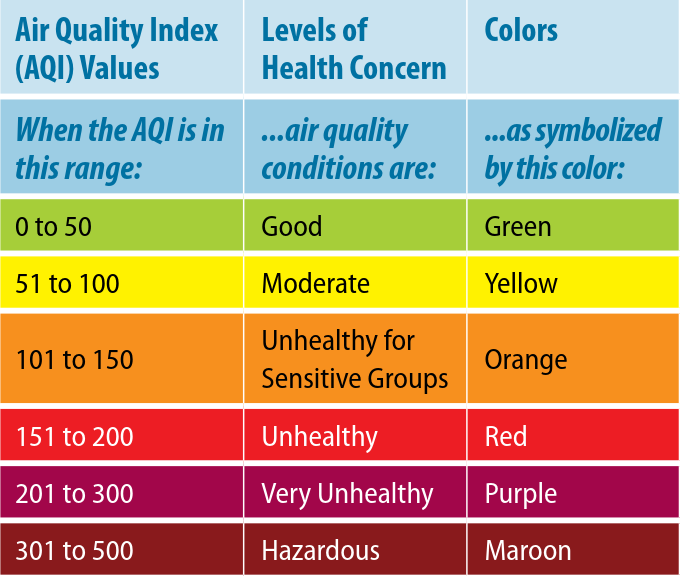
\includegraphics[scale=0.5]{aqi.png}
\caption{AQI Levels}
\label{fig:aqiLevels}
\end{figure}


